% \begin{figure}
%     \centering
%     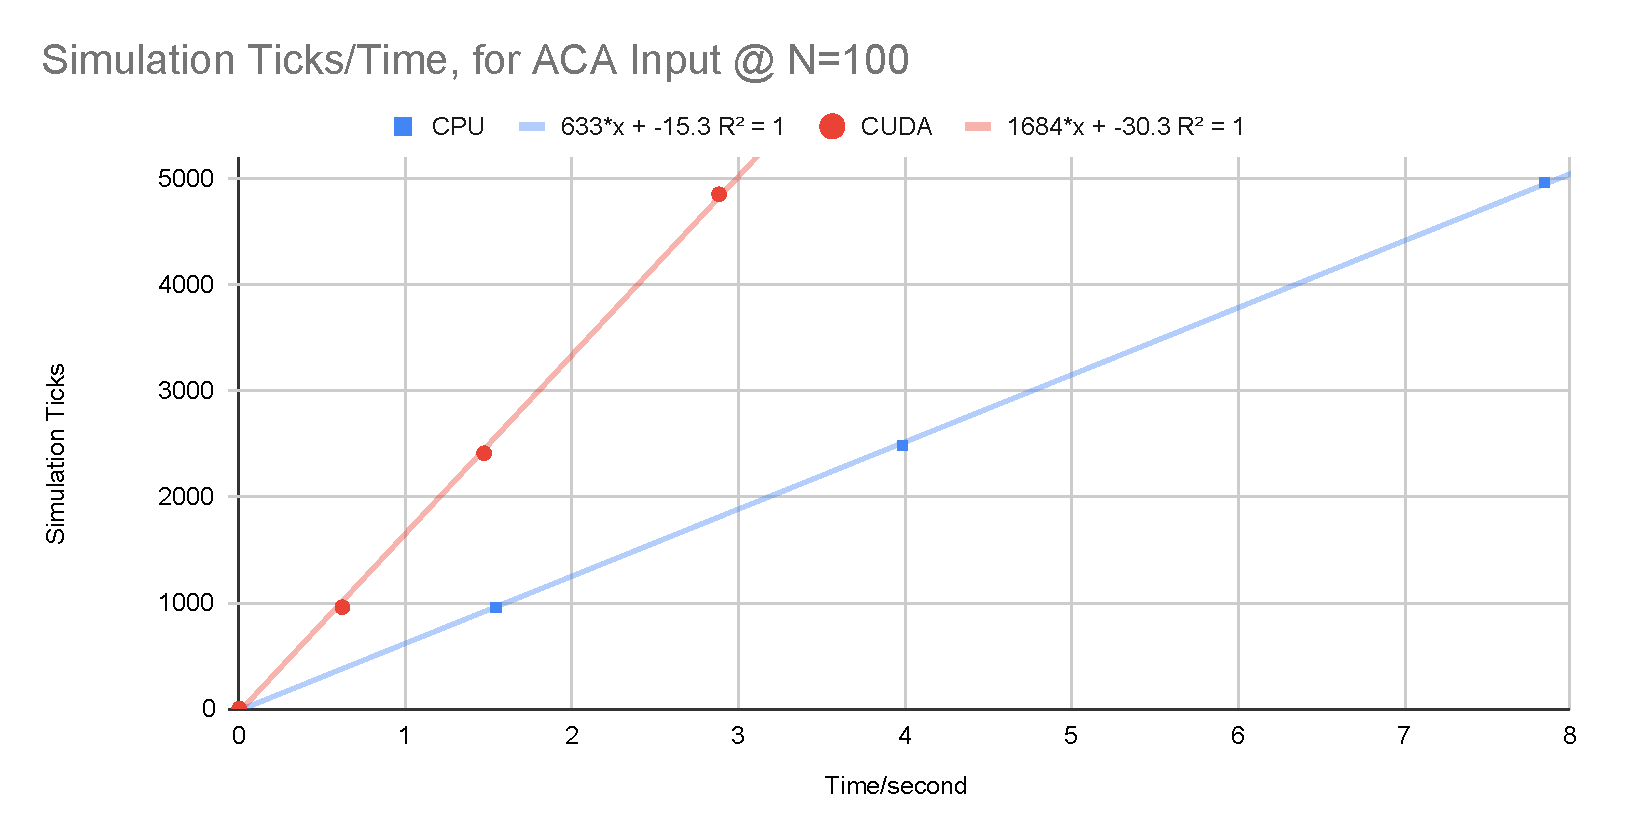
\includegraphics[width=\linewidth]{Ch62Results/figures/temp_ticks_vs_time_aca.pdf}
%     \caption{Ticks executed over time}
%     \label{fig:results:ticks_vs_time}
% \end{figure}

\begin{figure}
    \centering
    \begin{tikzpicture}
    \begin{axis}[
        title={Ticks Executed over Time},
        ylabel={Ticks Executed},
        xlabel={Time (\si{\second})},
        width=\linewidth,
        height=15em,
    ]
    \addplot table [x=Time, y=ticks_cpu, col sep=space, ignore chars={\,}] {Ch62Results/figures/data/time_ticks_cpu.csv};
    \addlegendentry{CPU};
    
    \addplot table [x=Time, y=ticks_cuda, col sep=space, ignore chars={\,}] {Ch62Results/figures/data/time_ticks_cuda.csv};
    \addlegendentry{CUDA};

    \end{axis}
    \end{tikzpicture}
    \caption{Ticks executed over time}
    \label{fig:results:ticks_vs_time}
\end{figure}